\documentclass[12pt,fleqn]{article}

\usepackage{amsmath}
\usepackage{amsthm}
\usepackage{amssymb}
\usepackage{algorithm}
\usepackage{algorithmic}
\usepackage{tikz}
\usepackage{geometry}
\usepackage{enumerate}
\usepackage{listings}
\usepackage{pdfpages}
\usepackage{inconsolata}
\usepackage{xfrac}
\usepackage{bm}
\usepackage{subcaption}
\usepackage{titlesec}
\usepackage{hyperref}
\usepackage{parskip}
\usepackage{minted}
\usepackage{etoolbox}

\newcommand{\code}[1]{\texttt{#1}}
\renewcommand{\qedhere}{\tag*{$\blacksquare$}}
\renewcommand{\qedsymbol}{$\blacksquare$}
\definecolor{bg}{rgb}{0.95,0.95,0.95}
\patchcmd{\thebibliography}{\section*{\refname}}{}{}{}

\title{%
    Parallel Minimum Distance Query Among Convex Meshes \\
    \Large 15-418/618 Final Project Report, Spring 2023}
\author{Yufei Shi (yshi2) and Bo Ying Su (boyings)}
\date{May 4, 2023}
\geometry{left=2cm, right=2cm, top=2cm, bottom=2cm}



\begin{document}
\maketitle



\section{Summary}
We implementated a parallel algorithm for computing the minimum distance and point pair between convex meshes using CUDA. We also parallelized the lookup function for Axis-Aligned Bounding Box (AABB) Hierarchy using OpenMP to filter mesh pairs that are far away from each other before passing the meshes to our algorithm.
We measured the performance of our program on a variety of scenes and compared the speedup of various implementation over a sequential algorithm that checks every pair of triangles.


\begin{figure}[ht!]
    \centering
    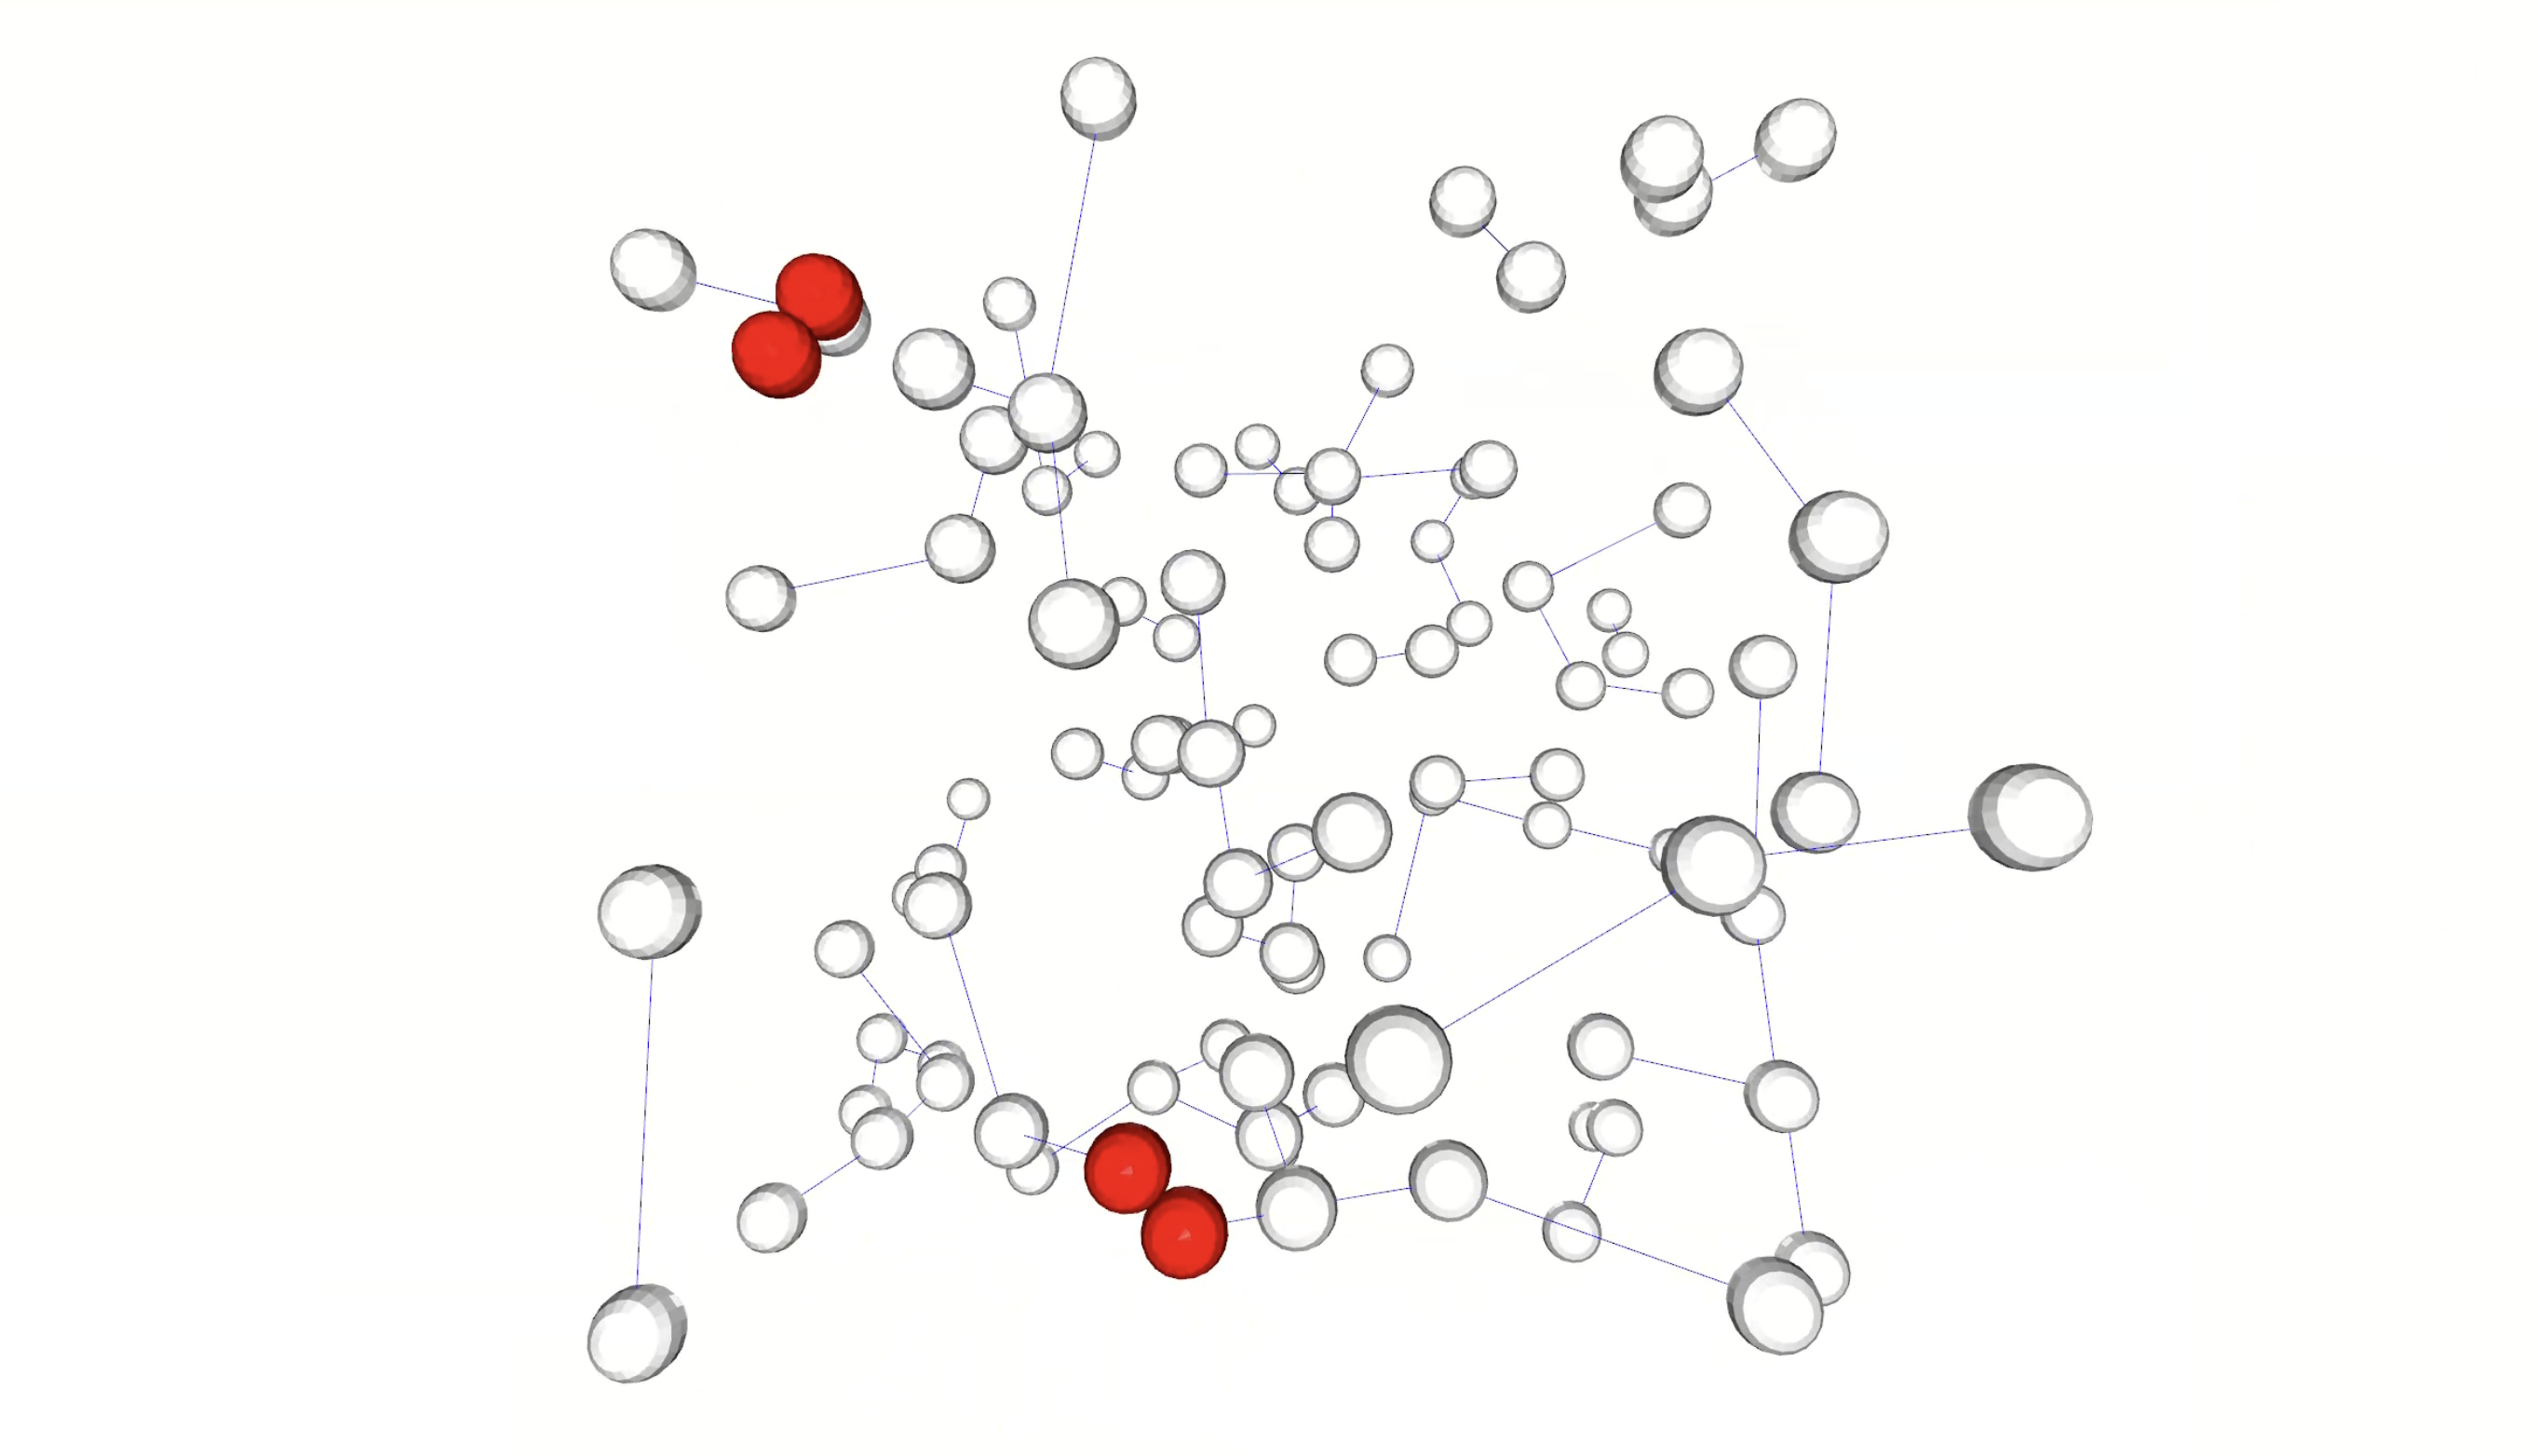
\includegraphics[width=1.0\textwidth]{figs/cover_new.png}
    \caption{%
            A screenshot of our program running on a scene with 19 meshes.
            Each mesh is connected to its nearest neighbor by a line segment.
            The red and blue line segments are produced by the sequential and parallel implementations, respectively.
            The collision pairs are marked in red.}
\end{figure}



% \pagebreak



\section{Background}
Collision detection and minimum distance query are fundamental problem in various fields, including computer graphics, robotics, and physical simulations.
The tasks in these fields require efficient and accurate collision detection to ensure the correctness of the simulation results.
Especially, in tasks such as robot motion planning, the collision detection algorithm must be able to handle complex interactions between multiple objects in real-time so that bad things (such as damaging the robot or the environment) do not happen. In the recent years, the development of Safety Set Algorithms (SSA) created a new demand for fast and accurate collision detection algorithms, due to its heavy use of minimal distance between object pairs in its control algorithm.
However, as the objects become more complex (more number of vertices) and the number of objects increases, the collision detection problem becomes more challenging as traditional sequential algorithms struggle to provide real-time performance.
This project aims to address this limitation by leveraging the power of parallel computing, using both CPU-based and GPU-based parallelism.


\subsection{Key Data Structures and Operations}
The problem we are trying to solve is basically two subproblems: finding close pairs and actually computing the minimum distance between the two meshes.
The first problem can be solved by iterating over all pairs of meshes and checking if they are close enough to each other. Or, we can use an AABB tree to filter out pairs of meshes that are far away from each other.
The second problem can be solved by the Naïve algorithm or using the GJK algorithm. Here we will briefly describe the key data structures and operations for these algorithms.


The most important data structure for our task is triangle mesh.
A triangle mesh is a collection of triangles that are connected to each other.
Normally, a triangle mesh also contains information about the color, texture, face normal, and other properties of the triangles.
However, for the purpose of collision detection, only the vertices and the connectivity information are needed.

In the naïve approach, we wrote a custom parser to load the triangle mesh from OBJ files.
Each mesh is represented as a list of vertices and a list of triangles faces (represented as indices of the vertices), as shown in the following code snippet.
\begin{minted}[bgcolor=bg, linenos]{c++}
struct Face { // triangle face, each face has 3 vertices
    int v1, v2, v3; // each vertex corresponds to an index in the vertices array
};

struct Mesh { // triangle mesh
    std::vector<Vec3> vertices; // Vec3 is a custom class, each contains 3 floats
    std::vector<Face> faces;
};
\end{minted}

We then determined that this is rather inefficient and switched to using the \code{Open3D} library to load the triangle mesh.
As an effect, we also had to switch to using the \code{Eigen} library for linear algebra operations.
The new key data structures are shown in the following code snippet.
\begin{minted}[bgcolor=bg, linenos]{c++}
class TriangleMesh() { // from Open3D, only key data structures are shown
public:
    std::vector<Eigen::Vector3d> vertices_;
    std::vector<Eigen::Vector3i> triangles_; // same as Face
    std::vector<std::unordered_set<int>> adjacency_list_; // connectivity info
};
\end{minted}

The GJK algorithm additionally requires a data structure called \code{simplex}, which is used to represent the current configuration of points that define the Minkowski difference of the two shapes being tested for collision.
The definition of \code{simplex} is shown below.
\begin{minted}[bgcolor=bg, linenos]{c++}
// [(vertex1, vertex2, lambda), ...]
typedef std::vector<std::tuple<int, int, double>> Simplex;
\end{minted}

The key operations that we need to perform on these data structures are computing the distance between any pair of triangles (naïve approach) and iteratively computing support points and searching for a simplex that encloses the origin (GJK algorithm).
These operations include computing using a subset of vertices, looping over all triangles, and a lot of vector operations.

In the late stage of the project, we also implemented an acceleration structure called Axis-Aligned Bounding Box (AABB) Hierarchy.
The key data structure for this algorithm is the AABB, which is a box that is aligned with the axes of the coordinate system~\cite{wikipedia_mbb,wikipedia_bvh}.
The definitions of \code{AABB, AABBTreeNode, AABBTree} are shown below.
\begin{minted}[bgcolor=bg, linenos]{c++}
class AABB {
public:
    int id; // id of the mesh (index in the list of meshes)
    Eigen::Vector3d minimum, maximum; // min and max coordinates
};
class AABBTreeNode {
public:
    AABB box;
    std::unique_ptr<AABBTreeNode> left, right; // children nodes
};
class AABBTree {
public:
    std::unique_ptr<AABBTreeNode> root;
};
\end{minted}

For \code{AABB}, we need to perform operations such as computing the bounding box given a mesh, checking intersection between boxes, and merging bounding boxes.
For \code{AABBTreeNode} and \code{AABBTree}, the key operations are building the tree and querying the tree for intersection.


\subsection{The Core Algorithm}

\subsubsection{Naïve Approach}
The naïve approach is to check every pair of triangles to see if they are colliding.
This works because the triangle meshes are convex, so if any pair of triangles are colliding, then the two meshes are colliding.
The collision check is done by computing the distance between the two triangles and checking if the distance is smaller than a threshold (0, in common case).
The triangle-to-triangle distance is in turn computed by taking the minimum of the distances between every pair of edges of the two triangles~\cite{larsen}.

This algorithm takes a list of meshes (each represented as a list of vertices and a list of faces) and returns the minimum distance between any pair of triangles.

\begin{algorithm}
    \caption{Naïve Algorithm}
    \begin{algorithmic}[1]
        \REQUIRE{$A$, $B$ : Convex shapes}
        \STATE Initialize $d_\text{min} = \infty$
        \FOR{triangle $a \in A$}
            \FOR{triangle $b \in B$}
                \STATE $d = \text{TriDist}(a, b)$ // triangle-to-triangle distance
                \IF{$d < d_\text{min}$}
                    \STATE $d_\text{min} = d$
                \ENDIF
            \ENDFOR
        \ENDFOR
        \RETURN $d_\text{min} \leq 0$
    \end{algorithmic}
\end{algorithm}

\subsubsection{Vanilla Sequential GJK Algorithm}
Since the naïve approach is very inefficient, we quickly switched to the Gilbert-Johnson-Keerthi (GJK) algorithm, which is the state-of-the-art algorithm for collision detection and minimum distance query between convex shapes~\cite{wikipedia_gjk}.

Given two convex shapes as input, the algorithm iteratively refines a simplex that approximates the solution.
The key idea behind GJK is the use of support functions to map the two shapes into a higher-dimensional space called the Minkowski difference, where the problem is transformed into finding the distance between the origin and the closest point in the Minkowski difference.
If the origin lies within this new space, it means the shapes intersect; otherwise, the algorithm outputs the points on the convex shapes that yield the minimum distance between them~\cite{cameron,serrano_2016}.

GJK begins by initializing a simplex with an arbitrary point in the Minkowski difference.
In each iteration, the algorithm finds the support point along the direction from the current closest point to the origin.
This support point is added to the simplex, and the simplex is then updated to its minimal subset containing the new support point that still encloses the origin.
The algorithm terminates when either the origin is found within the simplex or when the distance between the new support point and the current closest point is less than a predefined tolerance.
Upon termination, the output consists of points on the input convex shapes where the distance between them is the minimum distance between the two shapes~\cite{bittle_2010,10.5555/1121584}.
The GJK algorithm is highly efficient due to its linear complexity with respect to the number of dimensions and the number of vertices in the input shapes.

\begin{algorithm}
    \caption{GJK Algorithm}
    \begin{algorithmic}[1]
        \REQUIRE{$A$, $B$ : Convex shapes}
        \STATE Initialize simplex $S = \emptyset$
        \STATE Initialize $d = \text{arbitrary direction}$
        \WHILE{True}
            \STATE $p = \text{Support} (A, B, d)$
            \STATE Add $p$ to $S$
            \IF{$\text{dot}(p, d) \leq 0$}
                \RETURN False
            \ENDIF
            \IF{CheckTermination($S, d$)}
                \RETURN True // terminate if origin is in simplex, or if distance is small enough
            \ENDIF
        \ENDWHILE
    \end{algorithmic}
\end{algorithm}

This algorithm takes a list of meshes (each represented as a list of vertices and an adjacency list) and returns if there is a collision.
Additionally, GJK could also return the points on the two meshes that yield the minimum distance between them since the algorithm already computes them during the execution.

\subsubsection{Hill Climbing Sequential GJK Algorithm}
State-of-the-art GJK algorithms leverages the convex property of the input shapes to drastically improve the support function performance by using a hill climbing approach~\cite{cameron}. Give the previous support point, the algorithm can compute the next support point in the new direction in almost $O(1)$ time if the objects does not change its position or orientation too much. The function is defined in \ref{alg:hcsupport}. The hill-climbing optimization provide significant speedup. However, its sequential nature makes it hard to parallelize. Thus, we decided not to perform this optimization in our parallel algorithm.

\begin{algorithm}
    \caption{Support Algorithm}
    \begin{algorithmic}[1]
        \REQUIRE{$A$ : Convex shape, $d$ Direction}
        \FOR{vertex $v \in A$}
            \STATE $d = \text{dot}(v, d)$
            \IF{$d < d_\text{min}$}
                \STATE $d_\text{min} = d$
                \STATE $p = v$
            \ENDIF
        \ENDFOR
        \RETURN $p$
    \end{algorithmic}
    \label{alg:support}
\end{algorithm}

\begin{algorithm}
    \caption{Support Algorithm With Hill Climbing Optimization}
    \begin{algorithmic}[1]
        \REQUIRE{$A$ : Convex shape, $p$ Previous Support Vertex, $d$ Direction}
        \WHILE{$p$ is changing}
            \FOR{neighbors $b \in adjacency[p]$}
                \STATE $d = \text{dot}(b, d)$
                \IF{$d < d_\text{min}$}
                    \STATE $d_\text{min} = d$
                    \STATE $p = b$
                \ENDIF
            \ENDFOR
        \ENDWHILE
    \end{algorithmic}
    \label{alg:hcsupport}
\end{algorithm}

\subsubsection{Finding Close Pair Naïve Approach}
A naïve approach to finding pairs of meshes that is under a distance threshold is to perform a brute-force search. For each pair of meshes, we perform Axis-Aligned Bounding Box (AABB) intersection test. If the AABBs intersect, add them to the list. The algorithm is given by \ref{alg:naive_close_pair}.

\begin{algorithm}
    \caption{Finding Close Pair Naïve Approach}
    \begin{algorithmic}[1]
        \REQUIRE{$A$ : List of meshes, $d$ Distance Threshold}
        \FOR{$i \in A$}
            \FOR{$j \in A$}
                \IF{$i \neq j$}
                    \IF{$\text{AABBIntersection}(i, j)$}
                        \STATE $C \leftarrow C \cup \{(i, j)\}$
                    \ENDIF
                \ENDIF
            \ENDFOR
        \ENDFOR
        \RETURN $C$
    \end{algorithmic}
    \label{alg:naive_close_pair}
\end{algorithm}

\subsubsection{Finding Close Pair With Axis-Aligned Bounding Box (AABB) Tree}
Before we can perform the GJK algorithm on mesh pairs, we filter out pairs of meshes that are far away from each other by a given distance threshold. This is useful because in most of the use cases such as in robots, we care more about ensuring objects are far away from each other than a certain distance between them. By using an AABB tree, we can quickly filter out pairs of meshes that are not important, reducing the number of calls to the minimum distance query algorithm. The insertion function of the AABB tree is defined in \ref{alg:aabb_insert}. The query function is defined in \ref{alg:aabb_query}.


\begin{algorithm}
    \caption{AABB Tree Insertion}
    \begin{algorithmic}[1]
        \REQUIRE{$node$ : The node to insert into, $x$ the AABB to insert}
        \IF{$node$ is a leaf}
            \STATE replace $node$ with a new internal node with an AABB that encloses both $node$ and $x$, and two children $node$ and $x$
        \ELSE
            \STATE $branch\_cost \leftarrow \text{cost}(node \cup x) - \text{cost}(node)$
            \STATE $insert\_left\_cost \leftarrow \text{cost}(node.left \cup x) - \text{cost}(node.left)$
            \STATE $insert\_right\_cost \leftarrow \text{cost}(node.right \cup x) - \text{cost}(node.right)$
            \IF{$branch\_cost < insert\_left\_cost$ and $branch\_cost < insert\_right\_cost$}
                \STATE replace $node$ with a new internal node with an AABB that encloses both $node$ and $x$, and two children $node$ and $x$
            \ELSIF{$insert_left_cost < insert_right_cost$}
                \STATE $node.left \leftarrow \text{insert}(node.left, x)$
            \ELSE
                \STATE $node.right \leftarrow \text{insert}(node.right, x)$
            \ENDIF
        \ENDIF
        \STATE $node \leftarrow \text{update node AABB}$
        \RETURN $node$
    \end{algorithmic}
    \label{alg:aabb_insert}
\end{algorithm}

\begin{algorithm}
    \caption{AABB Tree Query} % finds all the potential collisions
    \begin{algorithmic}[1]
        \REQUIRE{$node$ : The node to traverse, $x$ the AABB to query}
        \IF{$node$ is a leaf}
            \STATE add $node$ to the list of potential collisions
        \ELSIF{$node$ intersects $x$}
            \STATE $\text{query}(node.left, x)$
            \STATE $\text{query}(node.right, x)$
        \ENDIF
    \end{algorithmic}
    \label{alg:aabb_query}
\end{algorithm}

\subsection{Workload Analysis}
In finding potential pairs of meshes to perform the minimum distance algorithm on, we can use a naïve approach of checking the bounding boxes of every pair of meshes. This approach has a time complexity of $O(n^2)$ where $n$ is the number of meshes. This is parallizable, as each pair of meshes can be checked in parallel. However, this approach has a poor locality since the meshes are stored in a list and the algorithm needs to loop through every other mesh in the list and compute the bounding boxes for any given mesh.
The other approach, where we use an AABB tree, has a time complexity of $O(n \log n)$ where $n$ is the number of meshes. The tree construction is inherently sequential, but the tree traversal can be parallelized. The tree traversal also has a poor locality since the tree is traversed in a depth-first manner. In summary, the naïve approach is more parallizable but has a worse sequential runtime, while the AABB tree approach has a better sequential runtime but is less parallizable. The trade-off analysis will be provided in the results section.

In querying the minimum distance between two meshes, we can use the naïve approach of computing the minimum distance between every pair of triangles. This approach has a time complexity of $O(n^2)$ where $n$ is the number of triangles in the two meshes. This approach is also parallizable, as each pair of triangles can be checked in parallel. However, this approach has a poor locality since the triangles are stored in a list and the algorithm needs to loop through every other triangle in the list and compute the minimum distance for any given triangle.
The other approach, where we use the GJK algorithm, has a time complexity of $O(n)$ where $n$ is the number of vertices in the two meshes. The algorithm is inherently sequential, but the support function can be parallelized. Additionally, many vector operations in GJK can be parallelized by precomputing a table of terms~\cite{bittle_2010}. This process has a good locality since the convex shapes and lists of support variables are stored in contiguous memory and are accessed often. In summary, the naïve approach is more parallizable but has a worse sequential runtime, while the GJK algorithm approach has a better sequential runtime but is less parallizable.

The loop of calculating the minimum distance between each pair of meshes is parallelizable, as there is no data dependency between each pair of meshes.

In general, the CPU parallelism is suitable for closest pair finding, while the GPU parallelism is suitable for minimum distance query.



% \pagebreak



\section{Approach}
In this section, we will describe the approach we took to implement the minimum distance query algorithm.

\begin{figure}[ht!]
    \centering
    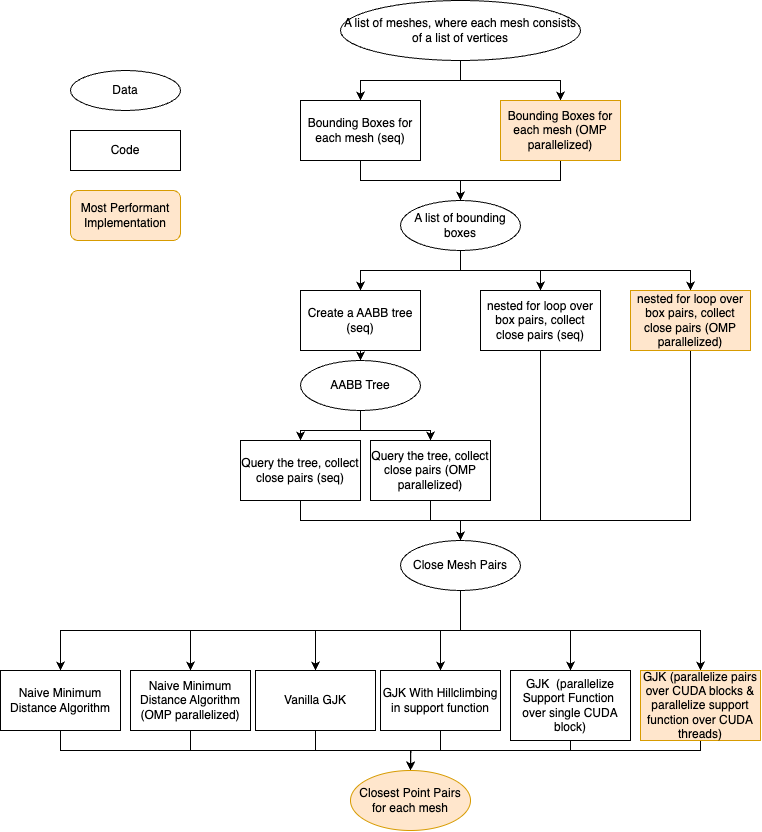
\includegraphics[width=1.0\textwidth]{figs/pipeline.drawio.png}
    \caption{%
            Our minimum distance over meshes pipeline. The program goes from the top to the bottom sequentially in each iterations. The rectangle blocks show possible implementations to select from. The color blocks are the best performance implementations we have found.}
\end{figure}

\subsection{Technologies Used}
Our main program is written in C++, leveraging the CUDA and OpenMP libraries for parallelization and Open3D and Eigen libraries for visualization and vector operations.
We use the CUDA library to perform GPU-based parallelism, and the OpenMP library to perform CPU-based parallelism.
We use the CMake build system to build our program.


\subsection{Mapping of the Algorithm to the Architecture}
\subsubsection{Parallelizing finding close pairs of meshes}
The purpose of finding close pairs of meshes is to filter out mesh pairs that are guaranteed to be far away from each other larger than a predefined threshold.
In the naive implementation of this function, we use a nested for loop to iterate over object pairs.
We parallelized it by using OpenMP.
We do not use CUDA to parallelize this function because the overhead of copying the data to the GPU is too large compared to the computation time.
In the AABB tree implementation, we use a recursive function to implement insert and query routines. They are kept sequential. However, we after the tree is constructed, we use OpenMP range-based parallelism to parallelize the queries over object pairs.

\subsubsection{Parallelizing Minimum Distance Query}
The goal is to leverage parallel computation to speed up finding the minimum distance between two meshes.
In the naive implementation, we have an outer loop that iterates over object pairs. Then we use a nested for loop to iterate over all pairs of triangles between the two meshes to find the minimum distance. We parallelized it by using OpenMP range-based parallelism.

In the GJK implementation, we parallelize the support function by leveraging CUDA threads. The support function finds the farthest point on the Minkowski difference of two convex shapes in a given direction. Since it calculates, and find the vertex whose dot product with the direction vector is the greatest, this makes a good case for parallelism. We parallelize the support function by assigning each CUDA thread to checking a single vertex, and find the maximum among them. We did not consider CPU parallelism since GJK runs in a loop, and the overhead of synchronizing the threads at the end of each iteration would be too large.

In the GJK implementation, we also parallize the calculation of dot products, cross products and areas. We precompute a table of terms, parallelized over CUDA threads.

In the Batched GJK implementation, we parallelize over pairs of meshes. That is, we launch a kernel with the grid size being the number of pairs of meshes, and the block size being the number of threads per pair of meshes. The block size is a hyperparameter and has to be greater than 25 (we assign threads to the precomputation of the table of terms statically).

In summary, our parallelized GJK algorithm processes a list of pairs of mesh in a single kernel launch, parallelizing support function over vertices and vector calculations over CUDA threads.

\begin{figure}[ht!]
    \centering
    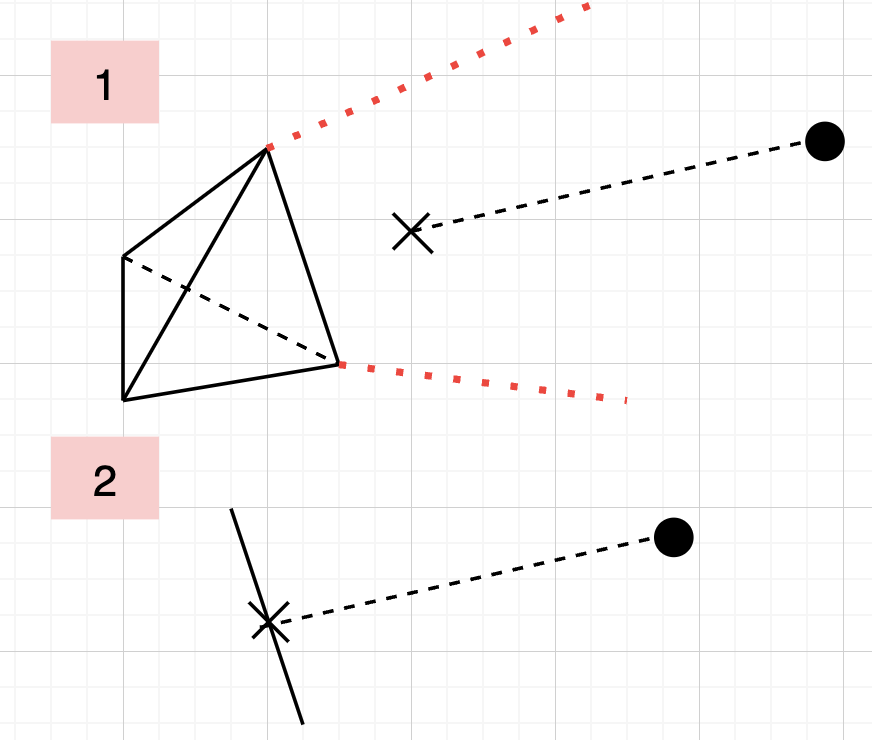
\includegraphics[width=0.3\textwidth]{figs/reduction.png}
    \caption{%
    In some iteration in the GJK algorithm, we try to find the minimum distance from the origin to the tetrahedron. The barycentric coordinate of the origin is calculated and the sign of its coefficients (commonly refered as lambda) determins which vonoroi region it is in. In this case, the origin is in the region belonging to the line segment on the right of the tetrahedron. The new simplex is the line segment on the right of the tetrahedron, and the new barycentric coordinate of the origin is again computed but instead based on the projection of the origin on the line segment. The new coefficients, which in this case are both positive, mean the projection of the origin lies on the line segment. The vector from the origin to the line segment is then use to update the new simplex point when calculating the support function in the next iteration.}
    \label{fig:reduction}
\end{figure}

\subsection{Optimizations Performed}
In the original GJK algorithm, the simplex is reduced one or most dimensions if its farthest vertex does not contribute to the projection of the origin to the simplex. This is done by calling one of the three recusive functions to reduce the simplex to a triangle, a line segment, or a point, depending on the location of the origin relative to the simplex. This introduces a lot of branches and conditional statements, which is not ideal for a parallel program. We optimized the routine of finding the closest point on the simplex to the origin by determining the vonoroi region of the origin using barycentric coordinates in a streamlined manner, inspired by~\cite{zhang2020barycode}. Our insight is that regardless which branch (simplex reduction) gjk takes, the simplex would only reduce its dimension strictly monotonically. Four conditional if statements, ordered by processing a tetrahedron, a triangle, a line segment, and a point, can cover all the possible paths that the reduction could take. \ref{fig:reduction} shows a case of a tetrahedron reduces to a point on a line.

Since calculating the barycentric coordinates requires a fixed set of dot product and cross product terms, we found that we can precompute a table of terms, leveraging the parallelism of CUDA threads. The actual calculation of the barycentric coordinates would then require just simple table lookups and additions.

\subsection{Referenced Code}
For the naïve approach, we referenced an implementation of the triangle-to-triangle distance algorithm~\cite{larsen}.
For the vanilla gjk implementation, we studied ~\cite{cameron} but we did not take code from them.

% \pagebreak


\section{Results}

\subsection{Definitions and Setup}
The performance of the algorithm is primarily measured by the time it takes to compute a correct result (if there is a collision, and the minimum distances between meshes).
This is wall-clock time.
The speedup of the parallel implementation is thus defined as the ratio of the time taken by the sequential implementation to the time taken by the parallel implementation.

The experiments are run on a machine with an AMD Ryzen 9 5900X 12-Core Processor and an NVIDIA GeForce RTX 3060 (with 12GiB device memory).
We have set up a few scenes with different number of kind of meshes to test the performance of different implementations.
The scenes are stored separately as configuration files in the \code{tests} directory so that the same scenes can be used for different implementations.
We also added an option in the framework to use a random scene generator to generate scenes that contains a given number of randomly places spheres.
The static scenes are used to analyze the performance of the algorithm with respect to the number of meshes, while the random scenes are used to analyze how the performance scales with respect to the number of meshes.

\subsection{Performance Analysis}
In this section, we discuss the effect of our optimizations on the performance of the algorithm.

\subsubsection{Parallelizing Close Mesh Pairs}
We first analyze the performance of the parallel implementation of the algorithm with respect to the number of meshes in the scene. The results are shown in \ref{fig:ablation_close_pair}. We observed that parallelizing the naive implementation of filtering with OpenMP yields the best result. We also profiled our AABB tree implementation and came to the conclusion that the overhead of building the tree (which is inherently not parallelizable) is too significant even when the query after it is fast.

The following summarizes the performance of the different implementations in a scene with 1000 meshes (sphere objects with radius 2 resolution 5):
\begin{itemize}
    \item Naive:                634560us (1x)
    \item Naive + OpenMP:       281005us (2.258180459x)
    \item AABB Tree:            3001880us (0.2113875305x)
    \item AABB Tree + OpenMP:   2053380us (0.3090319376x)
\end{itemize}

It can be seen that with high number of meshes in the scene, the Naive + OpenMP works the best.

The following summarizes the performance of the different implementations in a scene with 2 meshes (sphere objects with radius 2 resolution 1000):
\begin{itemize}
    \item Naive: 8us (1x)
    \item Naive + OpenMP: 21us (0.380952381x)
    \item AABB Tree: 23us (0.347826087x)
    \item AABB Tree + OpenMP: 20us (0.4x)
\end{itemize}

This is expected, as with small number of meshes, there is no parallelization opportunity here.


\subsubsection{Parallelizing Support Function in GJK}
The following summarizes the performance of the different implementations in a scene with 2 meshes (sphere objects with radius 2 resolution 1000):
\begin{itemize}
    \item CPU-Sequential: 12717400us (1x)
    \item CPU-Sequential-Hillclimb: 2566810us (4.954554486x)
    \item CPU-Parallel: 1248690us (10.18459345x)
    \item GPU-Sequential-support: 235575us (53.984506x)
    \item GPU-Parallel: 25758us (493.726221x)
\end{itemize}
From the experiment, we concluded that GPU-based parallelism works the best for support functions.


\subsubsection{Parallelizing Vector Calculations in GJK}
The following summarizes the performance of the different implementations in a scene with 2 meshes (sphere objects with radius 2 resolution 1000):
\begin{itemize}
    \item GPU-Vector-Sequential: 25118us (1x)
    \item GPU-Vector-Parallel: 21985us (1.142506254x)
    \end{itemize}
The numbers in this experiment fall within the error range. Thus, we conclude that the effect of parallelizing vector calculations is not significant.

\subsubsection{Parallelizing Processing Mesh Pairs}
In this section, we attempt to exploit the parallelization opportunity over mesh pairs. Note that the only difference of GPU-Sequential and GPU-Parallel is the number of blocks we launch at a time. The support function is still parallelized in GPU implementations.
The following summarizes the performance of the different implementations in a scene with 1000 meshes (sphere objects with radius 2 resolution 5):
\begin{itemize}
    \item CPU-Sequential: 34328600us (1x)
    \item CPU-Parallel: 3575860us (9.600096201x)
    \item GPU-Sequential: 1619300us (21.19965417x)
    \item GPU-Parallel: 1028300us (33.3838374x)
\end{itemize}

The following summerizes the performance of the different implementations in a scene with 5000 meshes (sphere objects with radius 2 resolution 5):
\begin{itemize}
    \item GPU-Sequential: 54142600us (1x)
    \item GPU-Parallel: 26261300us (2.061687731x)
\end{itemize}
Here we compare the effect of parallelizing over mesh pairs. That is, multiple GJK subroutines are launched in parallel. We see that CPU benefited hugely from this form of parallelization (our cpu hardware has 12 cores). However, in more extreme case with 5000 meshes, we observed that we can gain more speed up with parallelization with GPU on mesh pairs.



\subsubsection{Comparing Implementations}
Our analysis on the performance and speedup of the parallel implementation of the algorithm is done by using the same benchmark, \code{benchmark-lite}, which contains two meshes, each with 2404 faces.
The lite version of the benchmark is used because we wanted to include the performance of the naïve implementation as the baseline while not having to wait for a long time for the benchmark to finish.
Running this benchmark on the machine described in the previous section, we were able to generate the following plot.
\begin{figure}[ht!]
    \centering
    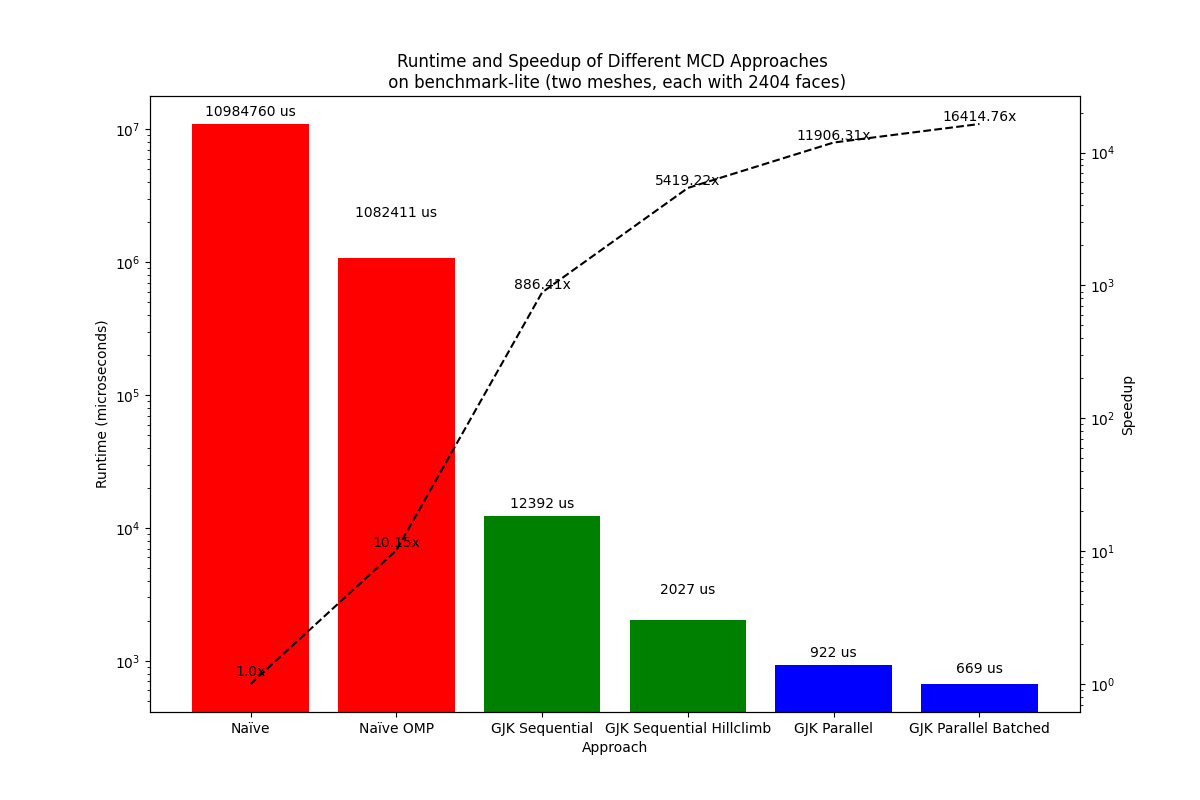
\includegraphics[width=0.95\textwidth]{figs/runtime_approaches.png}
    \caption{%
        Runtime and Speedup of Different MCD implementations.
        Implementations include Naïve, Sequantial GJK, and our Parallel GJK (and their optimized variants).
        The baseline, Naïve, is single-threaded CPU code.}
    \label{fig:runtime_approaches}
\end{figure}

In this plot, only Naïve, GJK Sequential, and GJK Sequential HillClimb are single-threaded CPU code.
Naïve OMP is an optimized version of the Naïve implementation using OpenMP.
GJK Parallel is an optimized parallel implementation for a single CPU based on GJK Sequential using CUDA.
GJK Parallel Batched is a further optimized version of GJK Parallel which uses multi-threading.

From the plot, we are able to observe good performance improvements through different parallelization techniques and the results are consistent with our expectation.
For example, the speedup of Naïve with OpenMP over Naïve is about 10x.
This is a reasonable number considering that the CPU has 12 physical cores and potential costs for managing and scheduling threads.
The speedup of the CUDA-parallelized GJK Parallel implementation over the GJK Sequential implementation is about 13.5x.
This is not as high as we initially expected.
But since GJK has some inherent sequential parts, it is not surprising that the speedup is not as high as we expected.

\subsection{Scalability Analysis}
We also analyzed the performance of the parallel implementation with respect to the number of meshes.
For this analysis, we used the random scene generator to generate scenes with 10, 100, 200, and 1000 randomly places spheres.
And for each scene, we ran the benchmark and recorded the average time taken by both the sequential and parallel implementations.
To fully test how well our implementation scales, we used the maximum dilation (i.e. \code{collision\_margin = $\infty$}), so that every possible pair of meshes is being checked by the algorithm, making the complexity to be in the order of $O(N^2)$.
\begin{figure}[ht!]
    \centering
    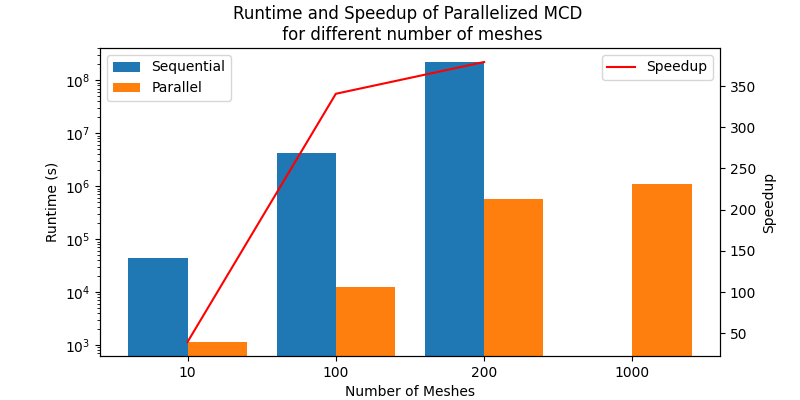
\includegraphics[width=0.95\textwidth]{figs/scalibility_approaches.png}
    \caption{%
        Runtime and Speedup of Parallelized MCD for different number of meshes.
        The runtime of sequential implementation for 1000 meshes is missing since it took too long for one iteration to finish.}
    \label{fig:scalibility_approaches}
\end{figure}

It could be observed that there is a diminishing return in the speedup as the number of meshes increases.
This is likely due to the fact that the complexity of the algorithm increases in the order of $O(N^2)$ (where N is the number of meshes), whereas the number of cores available on the GPU is only 3840.
So as the number of meshes increases, the program becomes more bounded by the limited resources (processing units and memory bandwidth) and the speedup does not increase as much as for the case with fewer meshes.

\subsection{Limitations and Deeper Analysis}

\subsubsection{Limitations of Our Parallel GJK Algorithm}
Our parallel implementation of the GJK algorithm requires the number of threads for each CUDA block to be greater than 25. This is purely due to programming though, as with some indexing effort, one could get around it.
Also, due to the algorithm is iterative and the result of each iteration is used to compute the next iteration, the SIMD parallelism is also not fully exploited as there could be divergence between threads in the same warp.

There are also some amounts of synchronization overhead in the parallel GJK implementation, which may also limit the performance of the parallel implementation.

\subsubsection{Reason Why the AABB Tree Implementation Does Not Work As Expected}
Our result show that the AABB tree implementation is slower than the naive implementation.
Our profiling result show that the tree insertion takes up most of the time and in the insertion function, code calculating the heuristic (either branching, inserting to the left, or inserting to the right) takes up most of the time.
Disabling the heuristic speeds up tree insertion by 2.23x but results in an unbalanced tree. The data structure construction itself is still a culprit of the slow down though, since without the heuristics the close mesh filtering is still around 4x slower than the naive implementation.

\subsubsection{Overhead of CPU and GPU Memory Transfer}
In cases where the number of meshes is large, the program will also become memory-bound as the GPU will start to run out of memory and extra time will be spent on transferring data between the host and the device.
We experimented in a scene consisting 1000 meshes (sphere objects with radius 2 resolution 5) with all the memory copying but without kernel launch.
We observed that it still results in 58133us latency, which is very significant.
This is with 42000 vertices.

\subsection{Choice of Machine Target}
Overall, we think that our choice of machine target (primarily GPU + some CPU) is sound.
The problem solution is highly data-parallel, involves a lot of vector operations, and its locality is fairly good.
These are all characteristics that are suitable for GPU-based parallelism.
Additionally, considering that it is likely to encounter scenes with a large number of meshes, the GPU is a good choice since it has a large number of cores that can be used to process the meshes in parallel.



% \pagebreak


\section{References}
\bibliographystyle{plain}
\bibliography{references}


% \pagebreak


\section{Credits}
Both authors contributed equally.


\end{document}